%----------------------------------------------------------------------------
\chapter{Technologies}

I worked using tools from the JVM-ecosystem, focusing on the problem description's key values, modernity, compatibility and portability. As such, I avoided using deprecated programming structures and unstable dependencies wherever possible.
% Munkámat a JVM-ökoszisztéma eszközeivel végeztem, szem előtt tartva a kiírásban kulcsfontosságú elemként rögzített modernitást, a kompatibilitást és a hordozhatóságot. Ennek megfelelően ahol lehetséges, kerültem a jövőbeli eltávolításra kijelölt programelemek használatát, illetve az instabil verzióktól függést.


\section{Kotlin \raisebox{-1ex}{\hspace{1cm}
\includegraphics[height=8mm, keepaspectratio]{images/kotlin_logo.png}}}

Kotlin is a multiplatform, statically typed, multi-paradigm programming language. Its specification is publicly accessible and updated regularly by JetBrains employees.~\cite{KotlinSpec} The first prototype was release in 2011, and the code was open sourced just a year later. The first full release of the language was published in 2016; since 2017, Android officially supports the it, and Android development has been code-first since 2019.~\cite{KotlinPast}

%A Kotlin multiplatform, statikusan típusos, több paradigmát támogató programozási nyelv. Specifikációját a JetBrains rendszeresen frissített, publikus, bárki által megtekinthető formában teszi közzé.~\cite{KotlinSpec} Az első prototípus verzió 2011-ben került kiadásra, és mindössze egy évvel később nyílt forráskódú projektté alakult. Az első éles kiadását 2016-ban érte el a nyelv, 2017-től hivatalosan támogatott az Android mobil operációs rendszerre írt alkalmazások terén, 2019 óta pedig az Android elsődleges nyelve.~\cite{KotlinPast}

Most of its popularity can be attributed to its intuitive syntax and near-perfect compatibility with JVM\footnote{JVM: \@Java Virtual Machine, a fully specified runtime currently owned by Oracle, mainly intended to run programs written in Java}. Any Java code can be referenced in a Kotlin program, allowing the use of countless Java community libraries. There is no restriction on the ratio of source files written in the two languages. It is worth noting however, that this compatibility is unidirectional -- Java code can not call Kotlin code.
%Népszerűségét elsősorban az intuitív szintaxisának és a JVM-mel\footnote{JVM: \@Java Virtual Machine, jelenleg az Oracle tulajdonában lévő, szabvánnyal specifikált futtatómotor, elsősorban a Java nyelven írt programok futtatásához } való már-már tökéletes kompatibilitásának köszönheti. Bármilyen Java-ban írt kódrészlet felhasználható külső referenciaként egy Kotlin programban, a programozó közösség által készített számtalan Java könyvtár így kiaknázható marad.  Egy projekten belül nincs korlátozás a két nyelv forrásfájljainak megoszlására; érdemes viszont megjegyezni, hogy a kompatibilitás egyirányú. Java kódból nem lehet visszahívni Kotlin kódba.

Finished programs go through compile and optimisation phases before they are turned into executable applications or libraries. Binaries made with Kotlin's compiler have near-identical performance to their traditional JVM counterparts. There are non-JVM compile targets as well:
%A megírt programok fordítási és optimalizálási fázisokon mennek keresztül, mielőtt futtatható állományok vagy eszköztárak készülnek belőlük. A Kotlin fordítómotorjával készített binárisok közel azonos teljesítményűek hagyományos JVM megfelelőikhez képest. A JVM-en kívül más fordítási célok is léteznek:
\begin{itemize}
    \item Kotlin/Native (Stable since 2023, provides native solutions for many operating systems without the need for a virtual machine)
    \item Kotlin/JS (programs are compiled to JavaScript, creating an interpreted codebase from compile-ready one; ideal for web browsers)
\end{itemize}
%\begin{itemize}
    %\item Kotlin/Native (2023 óta stabil, számos operációs rendszerre biztosít natív, futtató virtuális gépet nem igénylő megoldást)
    %\item Kotlin/JS (a megírt kódot JavaScript-re fordítjuk, így egy fordítást igénylő nyelvből interpretált kódot készíthetünk; webböngészőhöz ideális)
%\end{itemize}

The language's code structure is simple, easy to understand and quick to write. A lot of the frustrating syntactic and technical elements from Java were skipped or built around -- I'll show examples for this and the functional paradigm's possibilities in code sections.

%A nyelv alapvetően egyszerű kódstruktúrájú, jól értelmezhető és gyorsan írható. Emellett a frusztráló, sok esetben hátráltató szintaktikai és programtechnikai elemek közül sokat elhagytak a fejlesztők -- erre és a funkcionális paradigma által nyújtott lehetőségekre a későbbiekben számos példát fogok mutatni kódrészleteken keresztül.

I used the newest (2.0.21) version for my thesis through JetBrains' own integrated developer environment, IntelliJ Idea. I targeted the Oracle OpenJDK distribution's 23rd main version. The program guarantees compatibility with past versions until 21 LTS\footnote{Long Term Support, in software development, a publisher's pledge to provide longer-lasting, multi year support for a release}, released in September 2023 -- this version loses support in 2028.~\cite{JavaRoadmap}
%Szakdolgozatom elkészítéséhez a legfrissebb, 2.0.21-es verziót használtam a JetBrains saját, IntelliJ Idea néven futó programján keresztül. A felhasznált JVM változat a legújabb stabilnak tekinthető 23-as főverzió Oracle OpenJDK implementációja; a szakdolgozat során elkészült program által garantált abszolút minimális verzió a 2023 szeptemberében kiadott 21-es LTS\footnote{Long Term Support, a szoftverfejlesztés körében a kiadó által az adott verzióval kapcsolatban vállalt hosszabb idejű, több éves támogatást jelent} változat, ennek a főágú támogatása 2028-ban ér véget.~\cite{JavaRoadmap}

\section{OpenGL \raisebox{-1ex}{\hspace{1cm}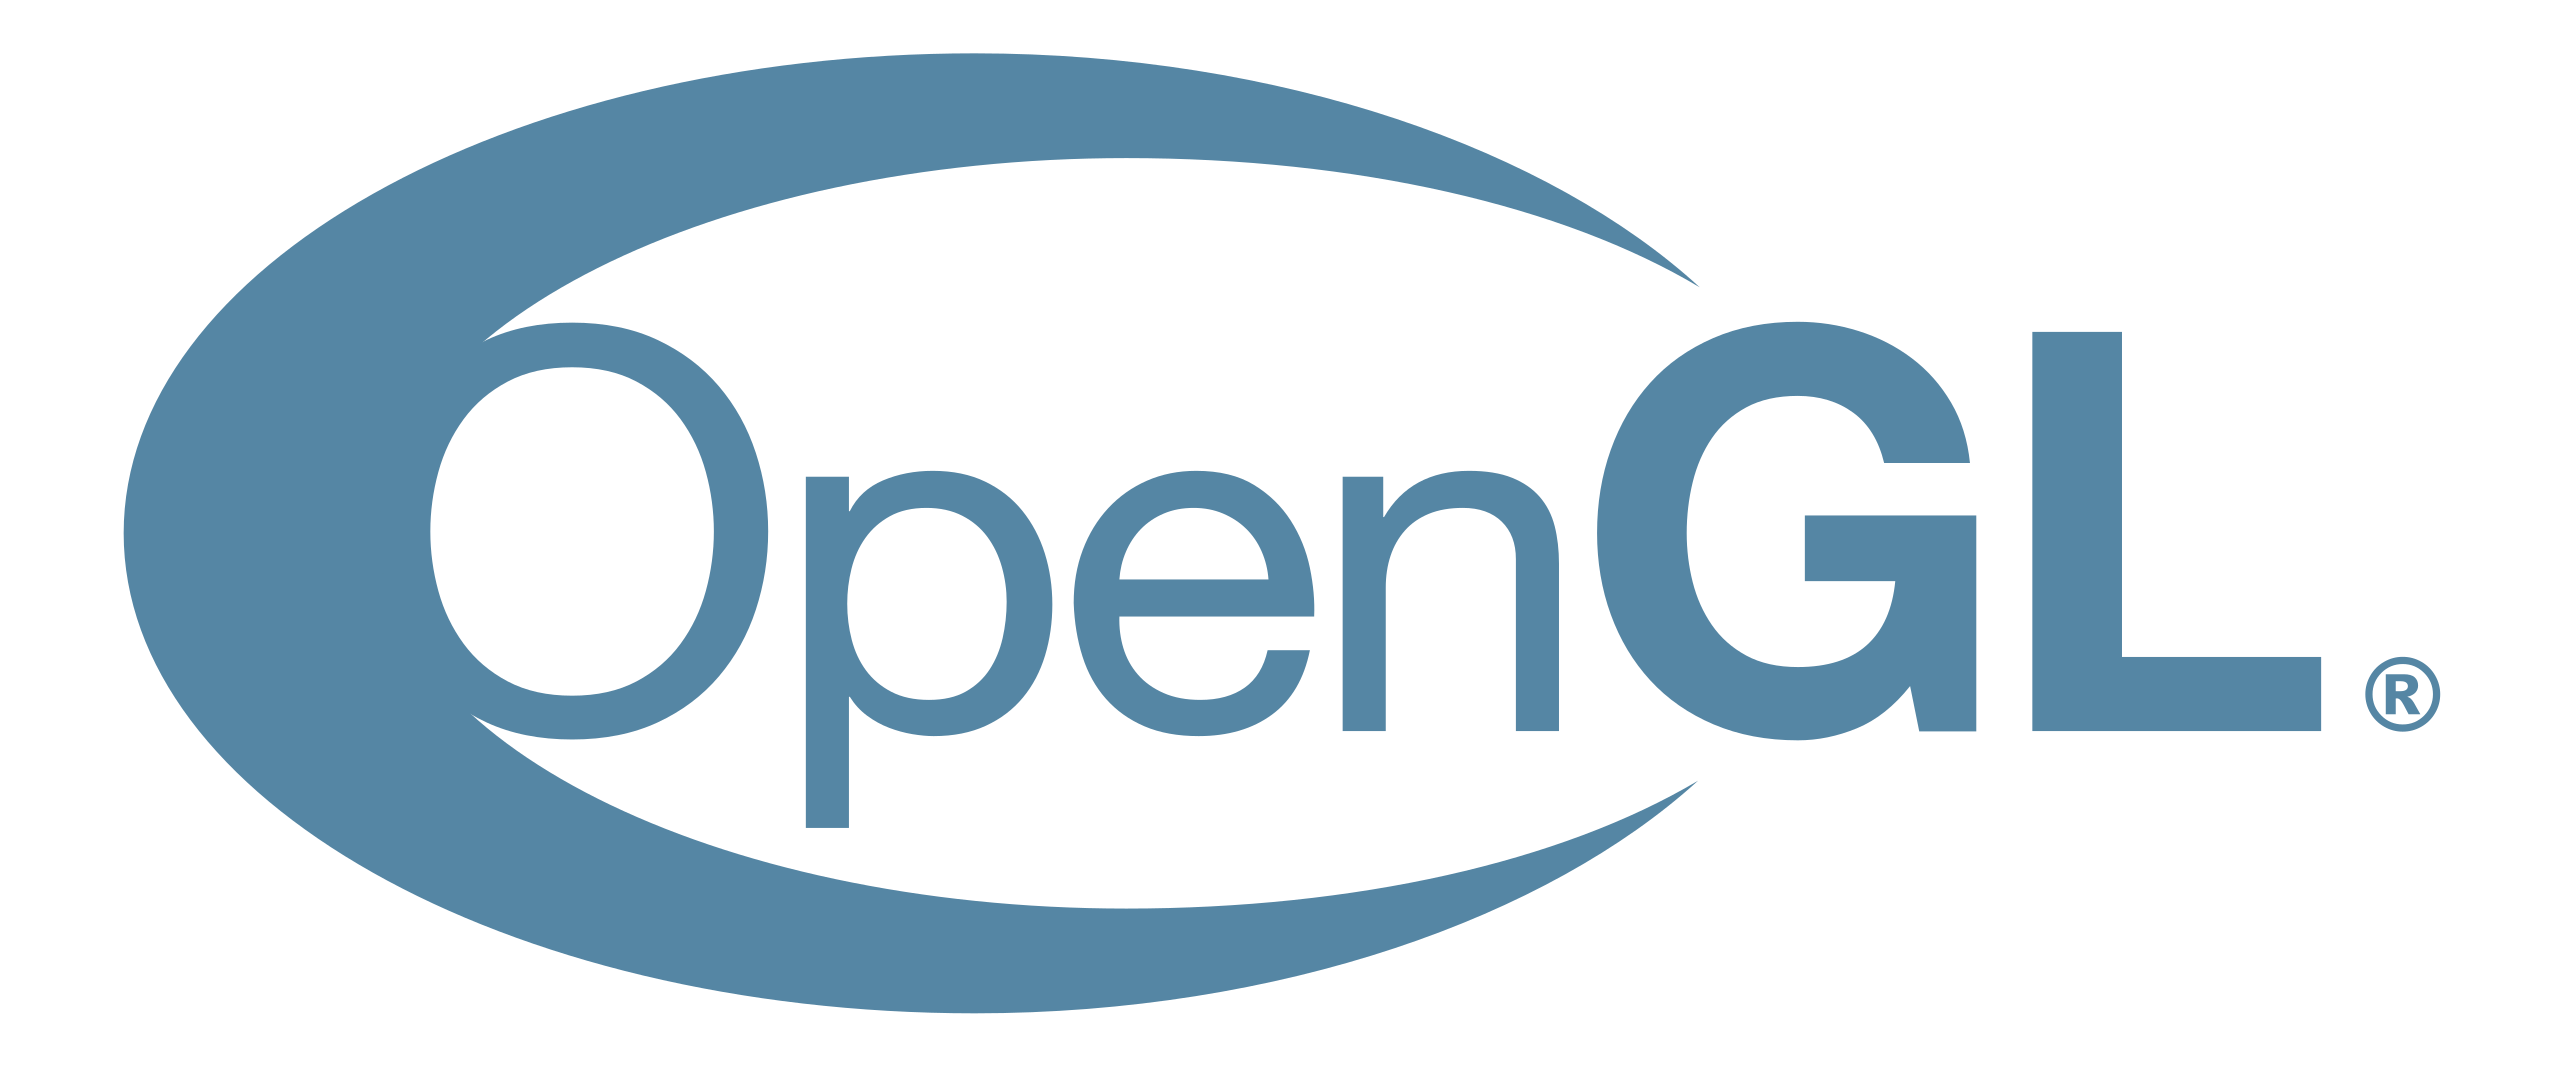
\includegraphics[height=8mm, keepaspectratio]{images/opengl_logo.png}}}

Popular low-level graphical library, capable of addressing the current screen down to the pixel level. It was first published in 1992, the newest version is 4.6, dating back to 2017 -- this is the single exception from my goals of using the latest tech.~\cite{OpenglHistory} OpenGL can be praised for its robustness and widespread support, the necessary graphics functions can be accessed on any operating system and by using nearly any programming language. Applications following the OpenGL standard can be expected to look identical on any system running it (provided the necessary dependencies are installed).

%Népszerű alacsony szintű grafikus könyvtár, amivel akár pixel szinten címezhető az éppen aktuális futtató felület. Első publikációja 1992-re tehető, a legújabb 4.6-os változat 2017-es dátumával ez a keretrendszer az egyetlen kivétel a modernitási törekvéseim alól.~\cite{OpenglHistory} Robosztussága és széles körű támogatottsága erős fegyvertény, hiszen szinte bármilyen nyelven és operációs rendszeren elérhetőek a kívánt grafikus függvények. Az OpenGL szabványnak megfelelő alkalmazásoknak ablakkezelő rendszertől függetlenül kiszámítható megjelenést kölcsönöz a szoftver.

\section{libGDX \raisebox{-0.1ex}{\hspace{1cm}
\includegraphics[height=6mm, keepaspectratio]{images/libgdx_logo.png}}}

LibGDX got the name from its multiple use cases: it's a "game development" and "effects" library for Java-based projects. It provides helper functions to make OpenGL operations callable in a JVM-idiomatic way, making it surprisingly easy to adjust graphics code to the style of the rest of the application.
%A libGDX nevét szerteágazó felhasználási lehetőségeiből kapta: "game development" és "effects" könyvtár Java alapú projektekhez. Segítségével az alacsony szintű OpenGL műveletek a JVM-környezetekre jellemző módon hívhatók meg, így meglepően jól illeszkedhet a grafikus felület kódja az alkalmazás többi részéhez.

Its predecessor was meant to aid the display of Android applications specifically. In 2010, the code was open sourced, creating the community-focused development of today.~\cite{LibgdxHistory} The current version number is 1.13.0. Created games and apps can be presented on desktop environments (Windows, macOS, Linux), mobile operating systems (Android, iOS) and even in most web browsers.
%Elődje kifejezetten Android alkalmazások megjelenítését segítette elő, 2010 óta közösségi támogatású, nyílt forráskódú eszközként fejlesztik.~\cite{LibgdxHistory} A projekt jelenlegi verziószáma 1.13.0; asztali környezetekben (Windows, macOS, Linux), mobil operációs rendszereken (Android, iOS) és webböngészőkben egyaránt prezentálhatóak az elkészült játékok.

\section{Exposed {\hspace{1cm}
\includegraphics[height=8mm, keepaspectratio]{images/exposed_logo.png}}}

Databases, specifically SQL\footnote{Structured Query Language, a domain-specific language used in the management of relational databases} have very old roots. Although the past decade saw many improvements - mainly with the release of developer-friendly tools - the standard's 40 years long history still strongly affects present-day programs.

%Az adatbázisok, azon belül az SQL\footnote{Structured Query Language, relációs adatbázisok kezeléséhez használt szakterület-specifikus nyelv} világa régi alapokon fekszik. Bár az elmúlt évtized is bővelkedik az újításokban - elsősorban fejlesztőbarátabb eszközök létrejöttével - a szabvány közel 40 éves története erősen kihat a mai felhasználásra.

The language's dialects are similar to regional accents, in a linguistic sense; a "speaker" of one variant may understand most or all other types, but that doesn't mean that they have the ability to correctly "express" themselves when using other types. There are multitudes of ORM\footnote{Object Relational Mapping, a technique intended to transform database records and in-memory objects into one another} libraries intended to bridge this gap. The most well-known ones include Hibernate for Java, EntityFramework for \.NET/\texttt{C\#}, and Active Record used in Ruby on Rails applications. The newly preferred Kotlin solution is Exposed, built mainly on JDBC (Java Database Connectivity). The library reflects Kotlin's philosophy of developer freedom -- data can be accessed in a classic object oriented manner, or through a custom language highly reminiscent of raw SQL.~\cite{ExposedDocs}

%A nyelv egyes dialektusai tulajdonképpen lingvisztikai tájszólásokhoz hasonlóak; az egyik típus "beszélője" a másikat is érteni fogja, de nem biztos, hogy "megszólalni" is helyesen tud. Ezeket az apró eltéréseket számos ORM\footnote{Object Relational Mapping, az adatbázisok és memóriában tárolt objektumok közötti átalakítás technikája} könyvtár kísérelte már meg áthidalni. Talán a legismertebb példák a Hibernate (Java), EntityFramework (.NET/\texttt{C\#}) és az Active Record (Ruby on Rails). A Kotlint fejlesztő JetBrains preferált megoldása a JDBC\footnote{Java Database Connectivity, kifejezetten a Java-hoz írt interfész réteg, célja minél több adatbázis formátum támogatása}-re épülő Exposed, ami tükrözi a Kotlin nagy szabadságot adó viselkedését. Hagyományos objektumorientált módon, avagy a nyers SQL-re nagyban hasonlító szabályokat használó, egyedi nyelvvel érhetjük el a tárolt adatokat.~\cite{ExposedDocs}

Portability is endorsed with database-agnosticism. Switching between supported database engines only requires changing a few configuration values -- this allows releasing our app with one of many implementations, from SQLite (popular on mobile) to Oracle Database (intended for multiple tenants and a highly distributed workflow).
%Nagy előny a hordozhatóság szempontjából az adatbázissal szembeni függetlenség: a támogatott motorok közötti váltás csupán egy konfigurációs érték módosítását igényli, így a mobilon jellemző SQLite-tól kezdve a szervereken átívelő redundáns Oracle Database implementációkig bármilyen környezetre alkalmas végterméket tudunk kiadni.

% TODO
\section{Ktor {\hspace{1cm}
\includegraphics[height=8mm, keepaspectratio]{images/ktor_logo.png}}}